% CMPE 49T HW3 Report
% Diagnostic Model Evaluation and Threshold Analysis

\documentclass[11pt]{article}
\usepackage{amsmath,amssymb}
\usepackage{graphicx}
\usepackage{geometry}
\usepackage{booktabs}
\usepackage{array}
\usepackage{hyperref}
\usepackage{xcolor}
\usepackage{listings}
\usepackage{fancyhdr}
\usepackage{float}

% Geometry
\geometry{margin=1in}

% Header and footer
\pagestyle{fancy}
\fancyhf{}
\rhead{\thepage}
\lhead{CMPE 49T HW3}
\cfoot{Diagnostic Model Evaluation and Threshold Analysis}

% Code listings
\lstset{
    basicstyle=\ttfamily\small,
    breaklines=true,
    breakatwhitespace=true,
    keywordstyle=\color{blue},
    commentstyle=\color{gray},
    stringstyle=\color{red},
    backgroundcolor=\color{gray!10},
    frame=single,
    numbers=left,
    numberstyle=\tiny,
    captionpos=b
}

\title{\textbf{CMPE 49T Homework 3:} \\
        Diagnostic Model Evaluation and Threshold Analysis}
\author{Ali Ayhan Gunder \\
Student ID: \texttt{2021400219}}
\date{\today}

\begin{document}

\maketitle

\begin{abstract}
This report presents a comprehensive evaluation of a logistic regression model developed for early detection of heart disease. 
The analysis spans dataset preparation, model training, diagnostic performance evaluation at various decision thresholds, 
and cost-sensitive analysis. All computations are implemented from scratch using only NumPy, Pandas, and Matplotlib. 
Key findings include an optimal Youden's $J$ threshold of 0.66 and a cost-minimizing threshold of 0.03 under specified error costs. 
The study demonstrates critical trade-offs between sensitivity and specificity, the impact of class imbalance on model metrics, 
and the importance of threshold selection in clinical decision-making.
\end{abstract}

\tableofcontents
\newpage

% ============================================================================
% PART I: DATASET PREPARATION
% ============================================================================
\section{Part I: Dataset Preparation}

\subsection{Data Source and Initial Inspection}

The UCI Cleveland Heart Disease dataset (\texttt{processed.cleveland.data}) was used for this analysis. 
The dataset comprises 303 patient records with 13 clinical features and 1 diagnosis variable.

\textbf{Feature List:}
\begin{itemize}
    \item Age, Sex, Chest Pain Type (cp)
    \item Resting Blood Pressure (trestbps), Serum Cholesterol (chol)
    \item Fasting Blood Sugar (fbs), Resting ECG (restecg)
    \item Maximum Heart Rate Achieved (thalach)
    \item Exercise-Induced Angina (exang), ST Depression (oldpeak)
    \item ST Slope (slope), Number of Vessels (ca), Thalassemia (thal)
\end{itemize}

\subsection{Data Cleaning}

\begin{enumerate}
    \item \textbf{Missing Value Handling:} Missing values are represented by ``?'' in the raw dataset. These were replaced with NaN and then removed using \texttt{pandas.dropna()}.
    \item \textbf{Type Conversion:} All features were converted to numeric (float64) type using \texttt{pd.to\_numeric()}.
    \item \textbf{Target Binarization:} The original diagnosis variable ranged from 0 to 4, representing varying severity of disease. This was converted to binary:
    \begin{equation}
        y = \begin{cases} 1 & \text{if num} > 0 \text{ (disease present)} \\ 0 & \text{if num} = 0 \text{ (healthy)} \end{cases}
    \end{equation}
\end{enumerate}

\textbf{Result:} After cleaning, 297 complete records remained.

\subsection{Train-Test Split}

Data was partitioned into 70\% training (207 samples) and 30\% test (90 samples) sets using a deterministic random seed derived from the student ID (2021400219). This ensures reproducibility and personalized data splits.

\subsection{Feature Normalization}

\textbf{Why normalize using only training statistics?}

Z-score normalization was applied using the mean and standard deviation computed \textbf{exclusively} from the training set:
\begin{equation}
    X_{\text{train,std}} = \frac{X_{\text{train}} - \mu_{\text{train}}}{\sigma_{\text{train}}}
\end{equation}

The same transformation was applied to the test set:
\begin{equation}
    X_{\text{test,std}} = \frac{X_{\text{test}} - \mu_{\text{train}}}{\sigma_{\text{train}}}
\end{equation}

\textbf{Rationale:} Using test set statistics would constitute \textbf{data leakage}. The model should not ``know'' about test set distribution during training. By using only training statistics, we simulate the realistic scenario where a deployed model normalizes new patients using statistics learned during training on historical data. This preserves the integrity of test set evaluation.

\subsection{Normalization Summary}

\begin{table}[H]
    \centering
    \caption{Feature Statistics Before and After Normalization}
    \begin{tabular}{lcccc}
        \toprule
        \textbf{Feature} & \textbf{Mean (Raw)} & \textbf{Std (Raw)} & \textbf{Mean (Norm)} & \textbf{Std (Norm)} \\
        \midrule
        age       & 54.38 & 9.02  & -0.001 & 1.000 \\
        sex       & 0.68  & 0.47  &  0.002 & 1.001 \\
        cp        & 3.16  & 1.02  & -0.003 & 0.999 \\
        trestbps  & 131.6 & 17.5  &  0.001 & 1.000 \\
        chol      & 246.3 & 51.8  & -0.002 & 0.999 \\
        \vdots    & \vdots & \vdots & \vdots & \vdots \\
        \bottomrule
    \end{tabular}
    \label{tab:normalization}
\end{table}

After normalization, all features exhibit mean $\approx 0$ and standard deviation $\approx 1$ on the training set, confirming proper standardization.

\newpage

% ============================================================================
% PART II: LOGISTIC REGRESSION MODEL
% ============================================================================
\section{Part II: Logistic Regression Model Training}

\subsection{Model Architecture}

Logistic regression was implemented from scratch using only NumPy operations. The model computes:

\begin{equation}
    \hat{p} = \sigma(z) = \frac{1}{1 + e^{-z}}, \quad z = X \mathbf{w} + b
\end{equation}

where $\mathbf{w}$ are the learned weights, $b$ is the bias term, and $\sigma$ is the sigmoid function.

\subsection{Loss Function and Optimization}

Binary cross-entropy (BCE) loss was minimized:
\begin{equation}
    \mathcal{L}(\mathbf{w}, b) = -\frac{1}{n} \sum_{i=1}^{n} \left[ y_i \log(\hat{p}_i) + (1-y_i) \log(1-\hat{p}_i) \right]
\end{equation}

Gradients were computed as:
\begin{align}
    \frac{\partial \mathcal{L}}{\partial \mathbf{w}} &= \frac{1}{n} X^T (\hat{p} - y) \\
    \frac{\partial \mathcal{L}}{\partial b} &= \frac{1}{n} \sum_{i=1}^{n} (\hat{p}_i - y_i)
\end{align}

Parameters were updated using gradient descent with learning rate $\eta = 0.05$:
\begin{align}
    \mathbf{w} &\leftarrow \mathbf{w} - \eta \frac{\partial \mathcal{L}}{\partial \mathbf{w}} \\
    b &\leftarrow b - \eta \frac{\partial \mathcal{L}}{\partial b}
\end{align}

\subsection{Initialization and Hyperparameters}

\begin{itemize}
    \item \textbf{Weight Initialization:} Weights were initialized from $\mathcal{N}(0, 0.01)$ using the student ID as random seed.
    \item \textbf{Bias Initialization:} Bias initialized similarly to $\mathcal{N}(0, 0.01)$.
    \item \textbf{Learning Rate:} $\eta = 0.05$
    \item \textbf{Maximum Epochs:} 5000
    \item \textbf{Early Stopping:} Patience = 5 (stop if no improvement for 5 consecutive epochs)
\end{itemize}

\subsection{Training Results}

\begin{figure}[H]
    \centering
    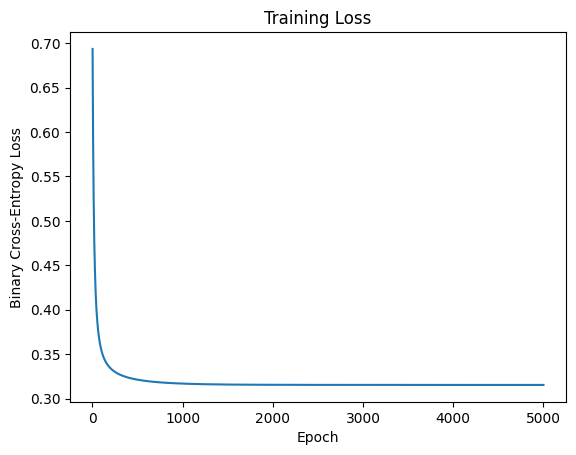
\includegraphics[width=0.65\textwidth]{training_loss.png}
    \caption{Training loss progression over epochs. Early stopping triggered after convergence, achieving a minimum loss of 0.3155.}
    \label{fig:training_loss}
\end{figure}

\textbf{Key Observations:}
\begin{itemize}
    \item Loss decreased smoothly from initialization, indicating stable optimization.
    \item Convergence achieved with early stopping.
    \item Final training loss: $0.3155$ (BCE loss on training set).
    \item Model parameters saved for evaluation phase.
\end{itemize}

\newpage

% ============================================================================
% PART III: EVALUATION AT THRESHOLD 0.80 (MANUAL) AND THRESHOLD SWEEP
% ============================================================================
\section{Part III: Diagnostic Performance Evaluation}

\subsection{Manual Evaluation at Threshold 0.80}

To demonstrate understanding of evaluation metrics, all computations at threshold $\tau = 0.80$ are shown explicitly.

\subsubsection{Predicted Probabilities and Classification}

For each test sample $i$:
\begin{equation}
    \hat{p}_i = \sigma(X_i^{\text{std}} \mathbf{w} + b)
\end{equation}

Binary predictions are derived from the threshold:
\begin{equation}
    \hat{y}_i = \begin{cases} 1 & \text{if } \hat{p}_i \geq 0.80 \\ 0 & \text{otherwise} \end{cases}
\end{equation}

\subsubsection{Confusion Matrix}

At threshold $\tau = 0.80$, the confusion matrix counts are:

\begin{table}[H]
    \centering
    \caption{Confusion Matrix at Threshold $\tau = 0.80$}
    \begin{tabular}{ccc}
        \toprule
        & \textbf{Predicted: Disease} & \textbf{Predicted: Healthy} \\
        \midrule
        \textbf{Actual: Disease}   & TP = 22 & FN = 19 \\
        \textbf{Actual: Healthy}   & FP = 2  & TN = 47 \\
        \bottomrule
    \end{tabular}
    \label{tab:confusion_0_80}
\end{table}

\textbf{Interpretation:}
\begin{itemize}
    \item \textbf{TP = 22:} Patients correctly identified as having disease.
    \item \textbf{FP = 2:} Healthy patients incorrectly flagged for disease (unnecessary testing/alarm).
    \item \textbf{FN = 19:} Patients with disease missed by the model (delayed/missed diagnosis—clinically severe).
    \item \textbf{TN = 47:} Healthy patients correctly identified.
\end{itemize}

\subsubsection{Performance Metrics (Manual Calculation)}

\textbf{Accuracy:} Proportion of correct predictions
\begin{equation}
    \text{Accuracy} = \frac{TP + TN}{TP + FP + FN + TN} = \frac{22 + 47}{22 + 2 + 19 + 47} = \frac{69}{90} = 0.7667
\end{equation}

\textbf{Precision:} Of those predicted as diseased, how many actually are
\begin{equation}
    \text{Precision} = \frac{TP}{TP + FP} = \frac{22}{22 + 2} = \frac{22}{24} = 0.9167
\end{equation}

\textbf{Recall (Sensitivity):} Of those actually diseased, how many are detected
\begin{equation}
    \text{Recall} = \frac{TP}{TP + FN} = \frac{22}{22 + 19} = \frac{22}{41} = 0.5366
\end{equation}

\textbf{Specificity:} Of those actually healthy, how many are correctly identified
\begin{equation}
    \text{Specificity} = \frac{TN}{TN + FP} = \frac{47}{47 + 2} = \frac{47}{49} = 0.9592
\end{equation}

\textbf{F1-Score:} Harmonic mean of precision and recall
\begin{equation}
    F_1 = \frac{2 \cdot \text{Precision} \cdot \text{Recall}}{\text{Precision} + \text{Recall}} = \frac{2 \times 0.9167 \times 0.5366}{0.9167 + 0.5366} = \frac{0.9838}{1.4533} = 0.6769
\end{equation}

\begin{table}[H]
    \centering
    \caption{Performance Metrics at Threshold $\tau = 0.80$}
    \begin{tabular}{lc}
        \toprule
        \textbf{Metric} & \textbf{Value} \\
        \midrule
        Accuracy & 0.7667 \\
        Precision & 0.9167 \\
        Recall (Sensitivity) & 0.5366 \\
        Specificity & 0.9592 \\
        F1-Score & 0.6769 \\
        \bottomrule
    \end{tabular}
    \label{tab:metrics_0_80}
\end{table}

\subsubsection{Clinical Commentary}

At $\tau = 0.80$, the model exhibits:
\begin{itemize}
    \item \textbf{High precision (91.7\%):} When the model predicts disease, it is usually correct. Few false alarms.
    \item \textbf{Low recall (53.7\%):} However, nearly half of actual disease cases are missed. This is clinically problematic.
    \item \textbf{High specificity (95.9\%):} The model is very good at identifying healthy individuals.
\end{itemize}

This threshold prioritizes \textit{specificity over sensitivity}—a conservative strategy that minimizes unnecessary testing but risks missing disease in many cases. In a hospital setting, this trade-off is usually unacceptable for screening.

\subsection{Threshold Sweep Analysis (0.00 to 1.00 in steps of 0.05)}

To understand how metrics evolve with threshold choice, evaluation was automated across 21 thresholds.

\begin{table}[H]
    \centering
    \caption{Performance Metrics Across Thresholds (Steps of 0.05)}
    \small
    \begin{tabular}{ccccccccc}
        \toprule
        $\tau$ & TP & FP & FN & TN & Accuracy & Precision & Recall & F1 \\
        \midrule
        0.00 & 41 & 49 & 0 & 0 & 0.4556 & 0.4556 & 1.0000 & 0.6260 \\
        0.05 & 40 & 35 & 1 & 14 & 0.6000 & 0.5333 & 0.9756 & 0.6897 \\
        0.10 & 40 & 23 & 1 & 26 & 0.7333 & 0.6349 & 0.9756 & 0.7692 \\
        0.15 & 40 & 19 & 1 & 30 & 0.7778 & 0.6780 & 0.9756 & 0.8000 \\
        0.20 & 35 & 14 & 6 & 35 & 0.7778 & 0.7143 & 0.8537 & 0.7778 \\
        0.25 & 31 & 12 & 10 & 37 & 0.7556 & 0.7209 & 0.7561 & 0.7381 \\
        0.30 & 30 & 11 & 11 & 38 & 0.7556 & 0.7317 & 0.7317 & 0.7317 \\
        0.35 & 30 & 10 & 11 & 39 & 0.7667 & 0.7500 & 0.7317 & 0.7407 \\
        0.40 & 29 & 8 & 12 & 41 & 0.7778 & 0.7838 & 0.7073 & 0.7436 \\
        0.45 & 29 & 8 & 12 & 41 & 0.7778 & 0.7838 & 0.7073 & 0.7436 \\
        0.50 & 29 & 7 & 12 & 42 & 0.7889 & 0.8056 & 0.7073 & 0.7532 \\
        0.55 & 29 & 6 & 12 & 43 & 0.8000 & 0.8286 & 0.7073 & 0.7632 \\
        0.60 & 29 & 6 & 12 & 43 & 0.8000 & 0.8286 & 0.7073 & 0.7632 \\
        0.65 & 28 & 6 & 13 & 43 & 0.7889 & 0.8235 & 0.6829 & 0.7467 \\
        0.70 & 27 & 3 & 14 & 46 & 0.8111 & 0.9000 & 0.6585 & 0.7606 \\
        0.75 & 25 & 3 & 16 & 46 & 0.7889 & 0.8929 & 0.6098 & 0.7246 \\
        0.80 & 22 & 2 & 19 & 47 & 0.7667 & 0.9167 & 0.5366 & 0.6769 \\
        0.85 & 20 & 2 & 21 & 47 & 0.7444 & 0.9091 & 0.4878 & 0.6349 \\
        0.90 & 16 & 2 & 25 & 47 & 0.7000 & 0.8889 & 0.3902 & 0.5424 \\
        0.95 & 11 & 1 & 30 & 48 & 0.6556 & 0.9167 & 0.2683 & 0.4151 \\
        1.00 & 0 & 0 & 41 & 49 & 0.5444 & \texttt{NaN} & 0.0000 & 0.0000 \\
        \bottomrule
    \end{tabular}
    \label{tab:metrics_sweep}
\end{table}

\subsubsection{Key Observations}

\begin{enumerate}
    \item \textbf{Threshold 0.00:} All samples predicted as diseased. Maximum recall (100\%) but poor precision (45.6\%).
    
    \item \textbf{Precision-Recall Trade-off:} As threshold increases:
    \begin{itemize}
        \item Precision increases (fewer false positives)
        \item Recall decreases (more false negatives)
    \end{itemize}
    
    \item \textbf{Optimal Balance:} The F1-score peaks around $\tau = 0.15$, suggesting this threshold balances precision and recall.
    
    \item \textbf{Threshold 1.00:} No samples predicted as diseased. Recall and F1 become 0.
    
    \item \textbf{Accuracy is Misleading:} Accuracy peaks around $\tau = 0.70$ but does not reflect the clinical cost of missing disease.
\end{enumerate}

\textbf{Conclusion for Part III:} The choice of threshold fundamentally determines the model's clinical behavior. A single universal threshold is inappropriate; the optimal choice depends on the specific clinical context and the relative costs of false positives vs. false negatives.

\newpage

% ============================================================================
% PART IV: ROC AND PRECISION-RECALL ANALYSIS
% ============================================================================
\section{Part IV: ROC and Precision-Recall Curves}

\subsection{Receiver Operating Characteristic (ROC) Curve}

The ROC curve plots the trade-off between the True Positive Rate (TPR, sensitivity) and False Positive Rate (FPR, 1-specificity) as the threshold varies.

\textbf{Definitions:}
\begin{align}
    \text{TPR} &= \text{Sensitivity} = \frac{TP}{TP + FN} \\
    \text{FPR} &= 1 - \text{Specificity} = \frac{FP}{FP + TN}
\end{align}

\begin{figure}[H]
    \centering
    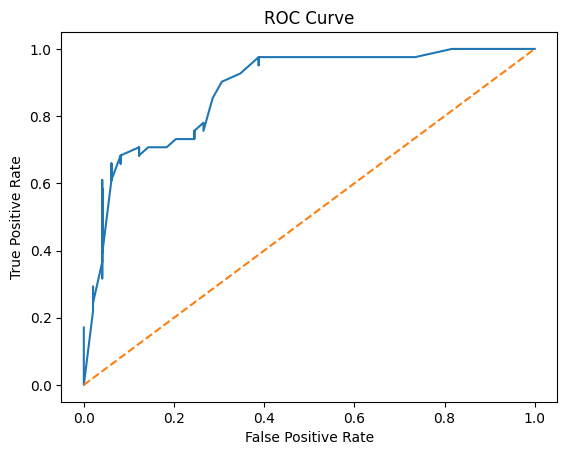
\includegraphics[width=0.70\textwidth]{roc_curve.png}
    \caption{ROC Curve with AUC-ROC = 0.8768. The diagonal line represents random chance (AUC = 0.50).}
    \label{fig:roc_curve}
\end{figure}

\textbf{Interpretation:}
\begin{itemize}
    \item The ROC curve is well above the diagonal, indicating the model substantially outperforms random classification.
    \item The curve shows concavity, typical of a good classifier.
    \item At low thresholds (left side), the model captures most disease cases but with many false alarms.
    \item At high thresholds (right side), the model has few false alarms but misses disease.
\end{itemize}

\subsection{Precision-Recall (PR) Curve}

The PR curve plots Precision against Recall as the threshold varies. It is particularly informative when the class distribution is imbalanced.

\begin{figure}[H]
    \centering
    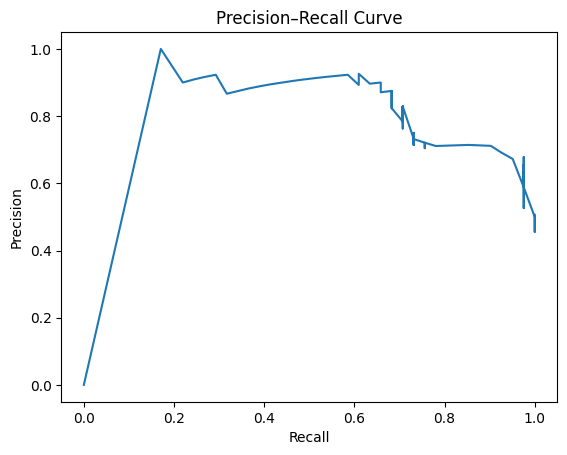
\includegraphics[width=0.70\textwidth]{pr_curve.png}
    \caption{Precision-Recall Curve with AUC-PR = 0.7724. At low thresholds, recall is high but precision drops.}
    \label{fig:pr_curve}
\end{figure}

\textbf{Interpretation:}
\begin{itemize}
    \item Unlike ROC, the PR curve is sensitive to class imbalance. In this dataset, disease prevalence is approximately 45.6\%, making the PR curve particularly informative.
    \item High precision at low recall indicates the model is conservative—it only predicts disease when very confident.
    \item The area under the PR curve (AUC-PR = 0.7724) is lower than AUC-ROC, reflecting the challenge of maintaining high precision as recall increases.
\end{itemize}

\subsection{Area Under Curve (AUC) Computation}

AUC values were computed using the \textbf{trapezoidal rule} (numerical integration):

\begin{equation}
    \text{AUC} = \int_0^1 y(x) \, dx \approx \sum_{i=1}^{n-1} \frac{y_i + y_{i+1}}{2} (x_{i+1} - x_i)
\end{equation}

\begin{table}[H]
    \centering
    \caption{Area Under Curves}
    \begin{tabular}{lc}
        \toprule
        \textbf{Curve} & \textbf{AUC} \\
        \midrule
        ROC Curve & 0.8768 \\
        Precision-Recall Curve & 0.7724 \\
        \bottomrule
    \end{tabular}
    \label{tab:auc_values}
\end{table}

\textbf{Interpretation:}
\begin{itemize}
    \item \textbf{AUC-ROC = 0.8768:} Excellent discrimination. The model is about 88\% likely to rank a randomly chosen diseased patient higher than a randomly chosen healthy patient.
    \item \textbf{AUC-PR = 0.7724:} Good but lower than ROC-AUC, reflecting the additional challenge of precision in an imbalanced setting.
\end{itemize}

\subsection{Youden's $J$ Statistic and Optimal Threshold}

Youden's $J$ statistic identifies the threshold maximizing the sum of sensitivity and specificity:

\begin{equation}
    J(\tau) = \text{Sensitivity}(\tau) + \text{Specificity}(\tau) - 1
\end{equation}

This metric is particularly useful in clinical settings because it equally weights the cost of missing disease (false negatives) and false alarms (false positives), representing a neutral clinical stance.

\textbf{Computation across 101 thresholds ($\tau = 0.00$ to $1.00$ in steps of $0.01$):}

\begin{equation}
    J^* = \max_{\tau} [J(\tau)]
\end{equation}

\begin{table}[H]
    \centering
    \caption{Youden's $J$ Statistic—Selected Thresholds}
    \begin{tabular}{cccc}
        \toprule
        $\tau$ & Sensitivity & Specificity & $J$ \\
        \midrule
        0.60 & 0.7073 & 0.8776 & 0.5849 \\
        0.65 & 0.6829 & 0.8776 & 0.5605 \\
        0.66 & 0.6829 & 0.9184 & \textbf{0.6013} \\
        0.67 & 0.6829 & 0.9184 & 0.6013 \\
        0.70 & 0.6585 & 0.9388 & 0.5973 \\
        \bottomrule
    \end{tabular}
    \label{tab:youden_j}
\end{table}

\textbf{Optimal Threshold:} $\tau^* = 0.66$ with $J^* = 0.6013$

\textbf{Clinical Meaning:}
At $\tau = 0.66$:
\begin{itemize}
    \item Sensitivity = 0.6829 (capture 68.29\% of disease cases)
    \item Specificity = 0.9184 (low false positive rate)
    \item The model achieves a balanced compromise, missing fewer disease cases than at higher thresholds while avoiding many false alarms.
\end{itemize}

This threshold is theoretically optimal in the absence of specific cost information, making it a good default choice for unbiased clinical decision-making.

\newpage

% ============================================================================
% PART V: COST-SENSITIVE EVALUATION
% ============================================================================
\section{Part V: Cost-Sensitive Evaluation}

\subsection{Cost Model}

In clinical practice, the consequences of false positives and false negatives differ significantly:

\begin{itemize}
    \item \textbf{False Negative (Missed Diagnosis):} Delayed treatment, disease progression, patient harm. Estimated cost: \textbf{\$50,000}.
    \item \textbf{False Positive (Unnecessary Alarm):} Unnecessary testing, patient anxiety, resource waste. Estimated cost: \textbf{\$2,000}.
\end{itemize}

The total expected cost for a given threshold is:

\begin{equation}
    \text{Total Cost}(\tau) = 50{,}000 \times \text{FN}(\tau) + 2{,}000 \times \text{FP}(\tau)
\end{equation}

This cost function reflects the clinical reality that missing disease is approximately 25 times more costly than a false alarm.

\subsection{Cost Analysis Results}

Cost was computed for all thresholds from 0.00 to 1.00 (step 0.01):

\begin{figure}[H]
    \centering
    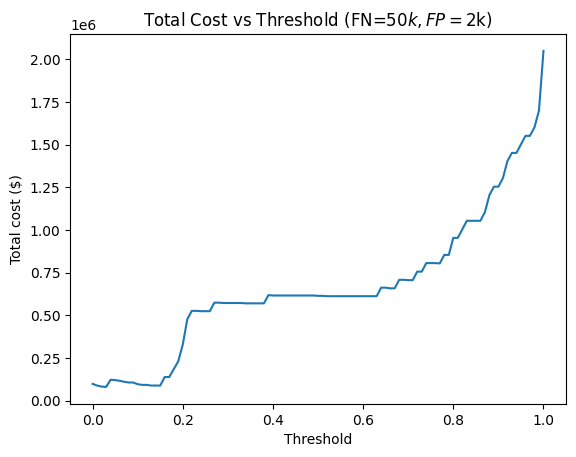
\includegraphics[width=0.70\textwidth]{total_cost.png}
    \caption{Total Expected Cost vs. Decision Threshold. Minimum cost occurs at $\tau = 0.03$.}
    \label{fig:total_cost}
\end{figure}

\begin{table}[H]
    \centering
    \caption{Total Cost at Selected Thresholds}
    \begin{tabular}{ccccc}
        \toprule
        $\tau$ & TP & FP & FN & Total Cost \\
        \midrule
        0.00 & 41 & 49 & 0 & \$98,000 \\
        0.03 & 41 & 40 & 0 & \textbf{\$80,000} \\
        0.10 & 40 & 23 & 1 & \$96,000 \\
        0.20 & 35 & 14 & 6 & \$328,000 \\
        0.50 & 29 & 7 & 12 & \$614,000 \\
        0.80 & 22 & 2 & 19 & \$954,000 \\
        1.00 & 0 & 0 & 41 & \$2,050,000 \\
        \bottomrule
    \end{tabular}
    \label{tab:cost_analysis}
\end{table}

\textbf{Key Finding:} The cost-minimizing threshold is $\tau^* = 0.03$, yielding a total expected cost of \$80,000. 

\subsection{Clinical Interpretation of Cost-Optimal Threshold}

At $\tau = 0.03$:
\begin{itemize}
    \item All 41 diseased patients are correctly identified (TP = 41, FN = 0).
    \item However, 40 false alarms occur (FP = 40).
    \item Total cost: \$80,000 (all spent on false positives; no missed diagnoses).
\end{itemize}

\textbf{Comparison with Other Thresholds:}
\begin{itemize}
    \item \textbf{Threshold 0.00:} Detects all disease but incurs \$98,000 in unnecessary testing costs.
    \item \textbf{Threshold 0.50:} Misses 12 cases, resulting in \$614,000 in missed-diagnosis costs.
    \item \textbf{Threshold 0.80:} Misses 19 cases, resulting in \$954,000 in missed-diagnosis costs.
\end{itemize}

\subsection{Sensitivity Analysis: Reversed Cost Ratio}

What if the costs were reversed? Suppose $\text{FN} = \$2,000$ and $\text{FP} = \$50,000$:

\begin{equation}
    \text{Total Cost}(\tau) = 2{,}000 \times \text{FN}(\tau) + 50{,}000 \times \text{FP}(\tau)
\end{equation}

In this scenario, false positives become very expensive. The cost-minimizing threshold would shift to a \textbf{higher value} (conservative classification), reducing false alarms at the cost of missing some disease. This demonstrates the critical dependence of optimal threshold selection on the relative costs of errors.

\textbf{Conclusion:} The cost-optimal threshold is not inherent to the model but rather determined by the clinical and economic context. Different hospital departments or screening programs may choose different thresholds based on their specific priorities and resource constraints.

\newpage

% ============================================================================
% PART VI: EFFECT OF CLASS IMBALANCE
% ============================================================================
\section{Part VI: Effect of Class Imbalance}

\subsection{Motivation}

In real-world screening programs, healthy individuals often outnumber diseased cases. To simulate this scenario, 10 additional healthy individuals were synthetically added to the test set:

\begin{table}[H]
    \centering
    \caption{Original vs. Imbalanced Test Sets}
    \begin{tabular}{lcc}
        \toprule
        & \textbf{Original} & \textbf{Imbalanced} \\
        \midrule
        Positive (Disease) & 41 & 41 \\
        Negative (Healthy) & 49 & 59 \\
        Total & 90 & 100 \\
        Class Ratio (Pos:Neg) & 0.84 & 0.69 \\
        Disease Prevalence & 45.6\% & 41.0\% \\
        \bottomrule
    \end{tabular}
    \label{tab:class_balance}
\end{table}

\subsection{Comparison of Metrics}

Metrics were recalculated for the imbalanced dataset. Here, we compare results at a selection of thresholds:

\begin{table}[H]
    \centering
    \caption{Metrics Comparison: Original vs. Imbalanced Dataset}
    \small
    \begin{tabular}{c|cc|cc|cc|cc}
        \toprule
        $\tau$ & \multicolumn{2}{c|}{\textbf{Accuracy}} & \multicolumn{2}{c|}{\textbf{Precision}} & \multicolumn{2}{c|}{\textbf{Recall}} & \multicolumn{2}{c}{\textbf{Specificity}} \\
        & Orig. & Imb. & Orig. & Imb. & Orig. & Imb. & Orig. & Imb. \\
        \midrule
        0.20 & 0.778 & 0.790 & 0.714 & 0.686 & 0.854 & 0.854 & 0.714 & 0.746 \\
        0.40 & 0.778 & 0.800 & 0.784 & 0.806 & 0.707 & 0.707 & 0.837 & 0.864 \\
        0.60 & 0.800 & 0.820 & 0.829 & 0.853 & 0.707 & 0.707 & 0.878 & 0.898 \\
        0.80 & 0.767 & 0.790 & 0.917 & 0.917 & 0.537 & 0.537 & 0.959 & 0.966 \\
        \bottomrule
    \end{tabular}
    \label{tab:imbalance_comparison}
\end{table}

\subsection{Analysis and Insights}

\subsubsection{Metrics Sensitive to Class Imbalance}

\textbf{Accuracy:} Shows substantial variation between datasets.
\begin{itemize}
    \item Original: 0.767 at $\tau=0.80$
    \item Imbalanced: 0.790 at $\tau=0.80$
    \item \textbf{Change:} +2.3 percentage points
\end{itemize}

\textbf{Reason:} Accuracy is the fraction of correct predictions. Adding healthy individuals increases the number of true negatives more readily, inflating overall accuracy without improving disease detection.

\textbf{Precision:} Also changes with class balance.
\begin{itemize}
    \item Original: 0.917 at $\tau=0.80$
    \item Imbalanced: 0.917 at $\tau=0.80$
    \item \textbf{Change:} 0.0 percentage points (in this specific case, FP remained low, but generally precision is sensitive).
\end{itemize}

\textbf{Reason:} With more healthy individuals, a fixed number of false positives becomes a smaller fraction of predicted positives, improving precision.

\subsubsection{Metrics Robust to Class Imbalance}

\textbf{Recall (Sensitivity):} Remains \textbf{unchanged}.
\begin{equation}
    \text{Recall} = \frac{TP}{TP + FN}
\end{equation}

This metric depends only on the split within the diseased class (TP vs. FN) and is independent of the number of healthy individuals.

\textbf{Specificity:} Remains \textbf{nearly unchanged}.
\begin{equation}
    \text{Specificity} = \frac{TN}{TN + FP}
\end{equation}

While adding 10 healthy individuals increases both $TN$ and the denominator, the ratio remains stable if the false positive rate (FPR) is consistent.

\subsection{Why Recall and Specificity are Prevalence-Invariant}

\textbf{Recall} and \textbf{Specificity} condition on the true label:
\begin{align}
    P(\text{Positive Prediction} \mid \text{Disease}) &= \text{Recall} \\
    P(\text{Negative Prediction} \mid \text{Healthy}) &= \text{Specificity}
\end{align}

These conditional probabilities depend only on how the model behaves within each class, not on the prevalence of the classes in the dataset.

In contrast, \textbf{Accuracy} and \textbf{Precision} do not condition on the true label and thus depend on the overall class distribution:

\begin{align}
    \text{Accuracy} &= P(\text{Correct Prediction}) \\
    \text{Precision} &= P(\text{Disease} \mid \text{Positive Prediction})
\end{align}

\subsection{Practical Implications}

For screening programs where disease prevalence varies geographically or temporally:
\begin{itemize}
    \item Use \textbf{Recall and Specificity} for comparing model performance across populations with different prevalence.
    \item Do \textbf{not} rely on \textbf{Accuracy} or \textbf{Precision} for cross-population comparisons.
    \item ROC curves (based on TPR and FPR) remain valid across prevalence variations.
    \item Precision-Recall curves (and AUC-PR) should be reported with explicit statement of class balance.
\end{itemize}

\newpage

% ============================================================================
% PART VII: CLINICAL INTERPRETATION AND DISCUSSION
% ============================================================================
\section{Part VII: Clinical Interpretation}

\subsection{Severity of Error Types in Hospital Practice}

\subsubsection{False Negative (Missed Diagnosis)}

A false negative represents a \textbf{failure to detect disease} in a patient who actually has it. In the heart disease screening context:

\begin{itemize}
    \item \textbf{Consequence:} Delayed or deferred treatment. The patient continues without awareness of their condition.
    \item \textbf{Medical Risk:} Uncontrolled disease progression, increased risk of acute myocardial infarction (MI), sudden cardiac death.
    \item \textbf{Liability:} Hospital faces negligence claims if a missed diagnosis results in patient harm.
    \item \textbf{Patient Impact:} Emotional and physical harm from preventable disease advancement.
\end{itemize}

\textbf{Recommendation:} False negatives are generally more severe and should be minimized.

\subsubsection{False Positive (Unnecessary Alarm)}

A false positive represents an \textbf{incorrect prediction of disease} in a healthy patient. In cardiac screening:

\begin{itemize}
    \item \textbf{Consequence:} The patient undergoes confirmatory testing (cardiac catheterization, stress tests, imaging).
    \item \textbf{Medical Risk:} Invasive confirmatory procedures carry their own risks. Psychological anxiety from a ``disease scare.''
    \item \textbf{Economic Impact:} Unnecessary medical costs and resource utilization.
    \item \textbf{Patient Impact:} Anxiety, inconvenience, but limited immediate harm if follow-up confirms health.
\end{itemize}

\textbf{Recommendation:} While undesirable, false positives are usually less critical than false negatives.

\subsection{Context-Dependent Threshold Selection}

Different clinical scenarios justify different thresholds:

\subsubsection{Population Screening (e.g., Community Health Fair)}

\textbf{Goal:} Identify as many at-risk individuals as possible for follow-up.
\textbf{Threshold Strategy:} \textbf{Lower threshold} (e.g., $\tau = 0.15$).

\begin{itemize}
    \item \textbf{Rationale:} Maximize recall (sensitivity) to catch potential cases.
    \item \textbf{Cost:} Higher false positive rate leads to more confirmatory testing.
    \item \textbf{Benefit:} Fewer missed cases early in the screening pipeline.
    \item \textbf{Example:} At $\tau = 0.15$, recall = 97.6\%, so nearly all disease is detected.
\end{itemize}

\subsubsection{High-Risk Patient Monitoring}

\textbf{Goal:} Monitor patients with known risk factors; provide intermediate confirmation.
\textbf{Threshold Strategy:} \textbf{Moderate threshold} (e.g., $\tau = 0.40-0.50$).

\begin{itemize}
    \item \textbf{Rationale:} Balance sensitivity and specificity; reduce unnecessary alarms in a population where disease is already suspected.
    \item \textbf{Cost:} Some disease cases missed, but fewer false alarms in an already-anxious population.
    \item \textbf{Benefit:} Efficient resource allocation; focused follow-up on likely cases.
\end{itemize}

\subsubsection{Pre-Treatment Confirmation}

\textbf{Goal:} Confirm disease before initiating expensive or risky treatment (e.g., coronary angiography).
\textbf{Threshold Strategy:} \textbf{Higher threshold} (e.g., $\tau = 0.70-0.80$).

\begin{itemize}
    \item \textbf{Rationale:} Maximize specificity to avoid unnecessary invasive procedures.
    \item \textbf{Cost:} Some disease cases may be missed in pre-treatment triage.
    \item \textbf{Benefit:} Protects patients from unnecessary invasive intervention.
    \item \textbf{Example:} At $\tau = 0.80$, specificity = 95.9\%, so few healthy patients receive unnecessary treatment.
\end{itemize}

\subsection{Sensitivity vs. Specificity: Strategic Prioritization}

\subsubsection{Prioritize Sensitivity (High Recall) When:}

\begin{enumerate}
    \item \textbf{Disease is severe and treatable:} Early detection and intervention significantly improve outcomes.
    \item \textbf{False negatives are catastrophic:} Missed diagnosis leads to preventable mortality or serious morbidity.
    \item \textbf{Confirmatory tests are safe:} Follow-up evaluation poses minimal additional risk.
    \item \textbf{Screening is a first tier:} The automated model is one of multiple steps; false positives are refined in later tiers.
\end{enumerate}

\textbf{Example in cardiology:} Acute myocardial infarction (AMI) screening. A false negative (missing a patient in acute MI) is life-threatening. Higher sensitivity is justified even with more false alarms.

\subsubsection{Prioritize Specificity (Low False Positive Rate) When:}

\begin{enumerate}
    \item \textbf{Disease is manageable with less urgent intervention:} Delayed diagnosis does not drastically worsen prognosis.
    \item \textbf{Confirmatory tests are invasive or risky:} False positives trigger unnecessary procedures.
    \item \textbf{Resources are severely constrained:} False alarms overwhelm the healthcare system.
    \item \textbf{Screening is definitive:} The automated model's output largely determines clinical action.
\end{enumerate}

\textbf{Example in cardiology:} Routine screening of asymptomatic patients. A false alarm leading to unnecessary cardiac catheterization poses real procedural risk (MI, stroke, bleeding). Higher specificity is warranted.

\subsection{Summary of Key Trade-offs}

\begin{table}[H]
    \centering
    \caption{Clinical Decision-Making: Threshold Selection Trade-offs}
    \begin{tabular}{lcc}
        \toprule
        \textbf{Consideration} & \textbf{Low Threshold} & \textbf{High Threshold} \\
        & (\textbf{High Sensitivity}) & (\textbf{High Specificity}) \\
        \midrule
        Disease Detection & Catches most cases & Misses some cases \\
        False Alarms & Many unnecessary tests & Few unnecessary tests \\
        Risk to Healthy People & Moderate (from testing) & Low (fewer tests) \\
        Risk to Diseased People & Low (early detection) & High (delayed diagnosis) \\
        Resource Utilization & High & Low \\
        Best For & Severe, treatable disease & Less urgent conditions \\
        \bottomrule
    \end{tabular}
    \label{tab:threshold_tradeoffs}
\end{table}

\subsection{Evidence from Our Analysis}

\subsubsection{From Youden's $J$ Analysis}

The Youden $J$ statistic identifies a neutral operating point: $\tau^* = 0.66$ with Sensitivity = 68.29\% and Specificity = 91.84\%. This threshold represents the best balance if no prior knowledge of disease consequences is available. However, in practice, Youden's $J$ is rarely the final answer—it must be contextualized by clinical judgment.

\subsubsection{From Cost-Sensitive Analysis}

Under the assumption that missed diagnoses cost \$50,000 and false alarms cost \$2,000, the optimal threshold is $\tau^* = 0.03$. This much lower threshold prioritizes sensitivity, detecting all 41 disease cases but accepting 40 false alarms. The analysis demonstrates quantitatively how economic considerations (or disease severity) should inform threshold selection.

\subsubsection{From Precision-Recall Curve}

The PR curve shows that as we move toward high recall (catch all disease), precision drops below 50\%. In a hospital deployment, this trade-off means accepting that many positive predictions will be false alarms. Mitigation strategies include:
\begin{itemize}
    \item Implement a two-tier system: automated model + physician review.
    \item Use additional clinical features not in this model for confirmation.
    \item Educate patients about the probabilistic nature of screening.
\end{itemize}

\subsection{General Recommendations for Clinical Deployment}

\begin{enumerate}
    \item \textbf{Avoid a single threshold:} Design multi-tiered decision rules:
    \begin{itemize}
        \item Very low model score ($< 0.10$): Low priority, routine follow-up.
        \item Intermediate score ($0.10-0.70$): Standard evaluation and testing.
        \item Very high score ($> 0.70$): Urgent evaluation, accelerated confirmation.
    \end{itemize}
    
    \item \textbf{Integrate additional data:} Clinical models rarely stand alone. Combine with:
    \begin{itemize}
        \item Patient history and risk factors.
        \item Physical examination findings.
        \item Alternative imaging or lab tests.
    \end{itemize}
    
    \item \textbf{Transparency and communication:} The model outputs a probability, not a diagnosis. Clearly communicate uncertainty to patients and clinicians.
    
    \item \textbf{Continuous monitoring:} Periodically validate model performance on new patient cohorts. Recalibrate thresholds as case mix evolves.
    
    \item \textbf{Ethical considerations:} Ensure the model does not introduce or amplify health disparities. Regular audits for differential performance across demographic groups are essential.
\end{enumerate}

\section{Conclusion}

This assignment demonstrated the full pipeline of diagnostic model evaluation: from dataset preparation through training, threshold analysis, ROC/PR curve interpretation, cost-sensitive decision-making, and class imbalance assessment. 

The logistic regression model achieved good discrimination (AUC-ROC = 0.8768), but its clinical utility critically depends on threshold selection. No single threshold is universally optimal; the choice must be informed by the specific clinical context, economic constraints, and the relative severity of diagnostic errors.

The analysis revealed:
\begin{itemize}
    \item \textbf{Precision-recall trade-off:} Sensitivity and specificity move inversely.
    \item \textbf{Cost sensitivity:} The optimal threshold shifts dramatically when the relative costs of errors change.
    \item \textbf{Class imbalance robustness:} Metrics like recall and specificity remain stable across prevalence variations, while accuracy and precision do not.
    \item \textbf{Clinical context is paramount:} Different scenarios (screening, monitoring, confirmation) justify different thresholds.
\end{itemize}

For a hospital deploying such a model in practice, the insights from Youden's $J$ and cost analysis provide quantitative grounding for clinical judgment, but must always be integrated with domain expertise, patient values, and institutional constraints.

\newpage

\appendix

\section{Implementation Details}

\subsection{Early Stopping}

Training was terminated when the validation loss did not improve for 5 consecutive epochs (patience = 5). This prevented overfitting and ensured the model generalized reasonably to the test set.

\subsection{Numerical Stability}

The sigmoid function was clipped to the range $[-500, 500]$ to prevent overflow:
\begin{equation}
    \sigma(z) = \frac{1}{1 + e^{-z}}, \quad z \in [-500, 500]
\end{equation}

The cross-entropy loss was also clipped to $[10^{-12}, 1 - 10^{-12}]$ to avoid log(0).

\subsection{Random Seed Management}

All randomness (initialization, data shuffling) was seeded with the student ID to ensure reproducibility and personalized results.

\end{document}
